\documentclass[../main.tex]{subfiles}
\begin{document}
\section{\label{sect:intro}Introduction}

%%%%%%%%%%%%%%%%%%%%%%%%%%%%%%
\subsection{The challenge of many-body quantum mechanics: memory and statistics}

In the early days of quantum mechanics it was quickly discovered that the Schr\"odinger equation could be solved analytically for hydrogen and hydrogen-like atoms in a straightforward manner~\cite{BetheSalpeterBook}. However, each new particle added to the problem came with a dauntingly steep price, leaving the vast majority of the periodic table of the elements unattainable due to the complexity of the equations and the accompanying high cost of computation. Indeed, the presence of more than two interacting particles yields equations that are analytically intractable; the quantum few-body problem thus appeared to be very difficult, and the chances of solving the quantum {\it many-body} problem seemed dire. At the heart of the problem is the fact that, while the influence of the massive atomic nucleus on the much lighter electrons can be approximated (as a static external field \`a la Born-Oppenheimer), addressing the Coulomb interaction among the electrons is far more challenging. Dirac famously remarked in 1929 that, while the underlying physical laws were then completely known, ``the difficulty is only that the exact application of these laws leads to equations much too complicated to be soluble''~\cite{DiracQuote}. This difficulty could hardly be overemphasized then, and remains a challenge to this day. In facing that challenge, a wide variety of algorithms was -- and continues to be -- developed by specialists around the world to fit the paradigms of their specific area of physics or chemistry.

The most common first-principles approaches to the quantum many-body problem can be roughly divided into two sets: memory intensive and statistics intensive. The former include methods such as exact diagonalization (see e.g.~\cite{BARRETT2013131,Johnson:2018hrx}) and coupled cluster (see e.g.~\cite{RevModPhys.79.291, Hagen:2013nca}), while the latter include a set of stochastic techniques generally known as quantum Monte Carlo (QMC) methods. Within that QMC set, this review focuses on a large class of approaches for which the many-body problem is expressed in the language of second-quantization or quantum field theory, such that expectation values of operators are written as a path integral over continuous fields living on a spacetime lattice. That formulation is in fact very general -- it is natural in relativistic quantum field theory as well as nuclear and condensed matter physics, either in the form of low-energy effective field theories (see e.g.~\cite{Burgess:2007pt,RevModPhys.81.1773,Machleidt:2011zz}), or as a reformulation of traditional Hamiltonians like the Hubbard model (see e.g.~\cite{Shankar:1996vk,doi:10.1142.6826}). Regardless of the application, the computational cost of path-integral QMC methods scales at face value (see below) polynomially with particle number and basis size (i.e. the size of the spacetime lattice), which makes them exceptionally well-suited for the many-body problem.

An essential component of QMC techniques is that they rely on a stochastic process governed by the Metropolis accept-reject algorithm~\cite{Metropolis}, which itself requires a well-defined probability measure to guarantee convergence to the correct result. Simply put, the algorithm requires that the
partition function $\mathcal Z$ be written as a sum of positive weights $W(C)$ (which play the role of the probability mentioned above) over some set of configurations $C$:
%
\beq
\mathcal Z = \sum_C W(C).
\eeq
%
The Metropolis algorithm, by construction, provides samples of the configurations $C$ distributed according to $W(C)$. Under many circumstances, however, a serious issue arises for this kind of algorithm, which has hindered computation in a wide range of situations: the infamous {\it sign problem}.
In those cases, $W(C)$ does not have a well-defined sign or even becomes complex (as explained in further detail below). Unfortunately, by far most systems of interest suffer from such a problem: high-$T_c$ superconductors (due to strong repulsive interaction away from half filling, see e.g.~\cite{PhysRevB.41.9301}), nuclear structure (strong repulsive core, finite spin-isospin polarization, see e.g.~\cite{KOONIN19971, Alhassid:2016ojg}), and quantum chromodynamics (finite quark density see e.g.~\cite{Gattringer:2016kco, Bongiovanni:2016ess, Aarts:2015tyj}), to name only a few.

Over the last few decades, many ideas have been proposed to overcome the sign problem in quantum many-body physics and field theory. This review covers some of them briefly and focuses on the so-called complex Langevin (CL) approach, as applied to the calculation of equilibrium properties of quantum many-body systems in relativistic and nonrelativistic physics, with an emphasis on the latter. The next section sketches out the basic path-integral formalism involved in Metropolis-based and stochastic quantization approaches, with the goal of showing where and how the sign problem arises.

%%%%%%%%%%%%%%%%%%%%%%%%%%%%%%
\subsection{Path integrals and the sign problem}

The central quantity of the field theoretical approach to the quantum many-body problem is the partition function,
which in the grand canonical ensemble is given by
%
\beq
\label{Eq:Z}
\mathcal Z = \textrm{Tr}\left[ {\rm e}^{-\beta (\hat H - \mu \hat N)} \right] ,
\eeq
%
where $\hat H$ is the Hamiltonian of the system, $\hat N$ the particle number operator, $\beta$ the inverse
temperature, $\mu$ the chemical potential, and the trace is over all multiparticle states (i.e. Fock space).
[Note that $\mathcal Z$ is shown here for a single particle species, but is straightforwardly generalized to multiple chemical potentials, etc.] As written, $\mathcal Z$ contains the thermodynamic information of the system: by differentiating with respect to $\beta$ and $\mu$ one obtains expectation values of the Hamiltonian and the particle number operators. More detailed information, such as momentum distributions and other correlation functions, can be obtained by adding sources to the Hamiltonian as is common in quantum field theory.

The direct evaluation of \equref{Z} is impossible for interacting systems, as it requires \textit{a priori}
knowledge of the full energy spectrum. The path-integral approach to the many-body problem
provides an alternative route. Either using an operator-based approach or coherent states, one
arrives at an expression for $\mathcal Z$ which is written generically as
%
\beq
\label{Eq:PartitionZ}
\mathcal Z = \int \mathcal D \phi\ {\rm e}^{-S[\phi]},
\eeq
%
where $\phi$ is a field living in $(d+1)$-dimensional spacetime and represents any degrees of freedom in the system.
One thus replaces the problem of evaluating \equref{Z} with that of calculating the above path integral.
In practice, boundary conditions in the spatial directions can be chosen in a variety of ways, but those in the time
direction, which is compact and runs in the range $\tau \in [0,\beta)$, are set by the quantum statistics of the problem:
bosonic fields will obey periodic boundary conditions and fermionic fields anti-periodic.

From this point on, our discussions will focus on nonrelativistic systems unless otherwise specified.
In purely bosonic theories the action $S[\phi]$ will typically take a simple local form such as
%
\beq
\label{Eq:BosonAction}
S[\phi] = \int \d\tau \d^dx \left\{ \phi^* \left (\partial_\tau + {\mathcal H}\right) \phi + V[\phi] \right\},
\eeq
%
where $\mathcal H$ represents the noninteracting Hamiltonian (including external trapping potentials) and $V[\phi]$ represents the interactions
(i.e. terms cubic and beyond in $\phi$).

For real bosonic variables $\phi$, the action $S[\phi]$ is also real and therefore ${\rm e}^{-S[\phi]}$ can be used as a probability measure in a stochastic process.
For complex $\phi$, however, the fact that $\partial_\tau$ is an antisymmetric operator results in a complex $S[\phi]$, which is the source of
a sign problem in this formulation (see below) and has a counterpart in relativistic bosons at finite chemical potential (see Secs.~\ref{sect:DualVariables} and~\ref{sect:RQFT}).
The problem of the antisymmetry of $\partial_\tau$ can be circumvented for an even number of species with attractive interactions,
which however render bosons unstable (but not fermions, see below).

\begin{figure}[h]
  \centering
  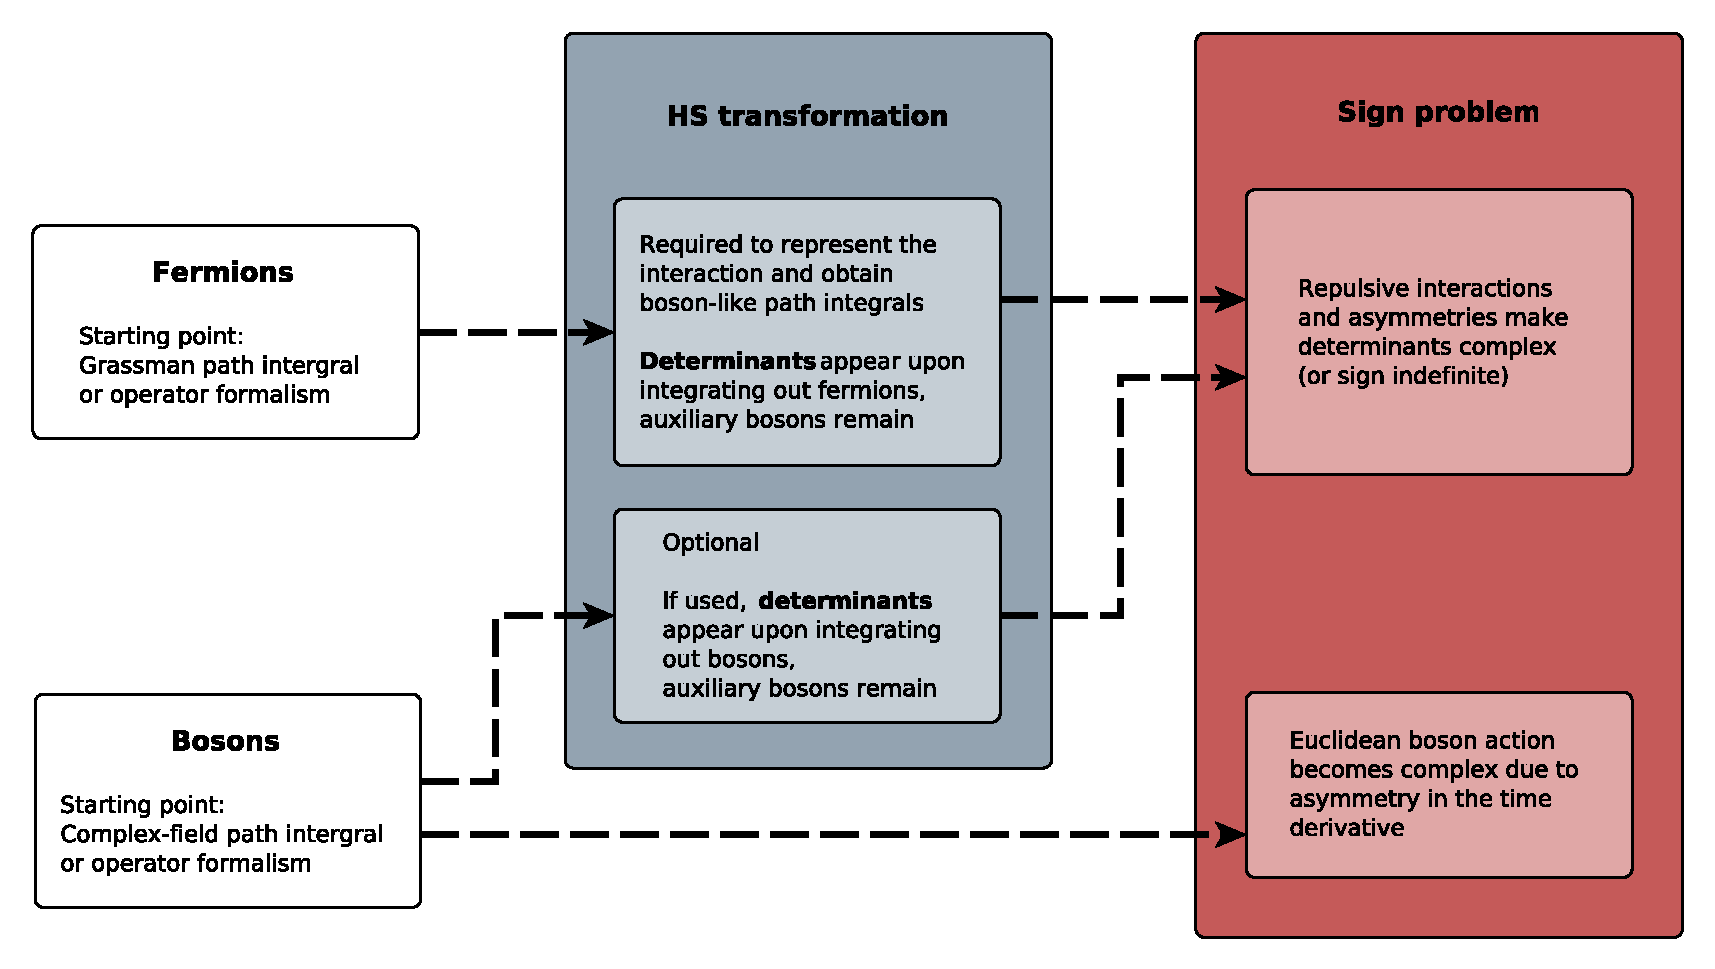
\includegraphics[width=\columnwidth]{./1introduction/sign_problem_graph.pdf}
  % \includegraphics[width=0.75 \columnwidth]{./1introduction/PathIntegralsFermionsBosons.pdf}
  \caption{\label{fig:PathIntegralsFermionsBosons} Pathways of the appearance of the sign problem in path-integral approaches to non-relativistic many-body systems.}
\end{figure}


To make contact with the fermionic case discussed below (see also \figref{PathIntegralsFermionsBosons}), it is instructive to rewrite the interaction using a Hubbard-Stratonovich (HS) transformation, although it is not strictly needed in the bosonic case. Consider for instance the case of a complex field $\phi$. Schematically, one introduces
an auxiliary field $\sigma$ such that
%
\beq
{\rm e}^{-S_{\rm int}[\phi]} =  \int \mathcal D \sigma\;  {\rm e}^{-S_{\rm aux}[\phi,\sigma] - S_{0}[\sigma]},
\eeq
%
where
%
\beq
S_{\rm int}[\phi] = \int \d\tau \d^dx\ V[\phi] \, ,
\eeq
%
$S_{\rm aux}[\phi,\sigma]$ is a quadratic functional of both $\phi$ and $\sigma$, and $S_{0}[\sigma]$ is a pure-$\sigma$ term; both $S_{\rm aux}$ and $S_{0}$ depend on the specific
choice of HS transformation. Since the action is now quadratic in $\phi$, the corresponding path integral can be carried out, which results in a $\sigma$-dependent determinant, i.e. the full partition function can now be expressed as
%
\beq
\label{Eq:PartitionZ}
\mathcal Z = \int \mathcal D \sigma \;  {\rm e}^{-S_{\rm HS}[\sigma]},
\eeq
%
where
%
\beq
\label{Eq:SHSBosonDeterminant}
{\rm e}^{-S_{\rm HS}[\sigma]} = \frac{{\rm e}^{-S_{0}[\sigma]}}{\det M[\sigma]}.
\eeq
%

Usually it is possible to factor the determinant into a determinant for each particle species (flavors), such that if $N_f$ flavors are present then
%
\beq
\label{Eq:BosonDeterminant}
\det M[\sigma] = \det M_1[\sigma] \det M_2[\sigma]\, \cdots\, \det M_{N_f}[\sigma].
\eeq
%
%
Naturally, calculations with bosons are not carried out using the action of \equref{SHSBosonDeterminant}.
Indeed, the formulation based on $S[\phi]$ of \equref{BosonAction} is considerably easier to work with as
there are no determinants involved. However, the appearance of the boson determinant in \equref{SHSBosonDeterminant}
shows that, if $\det M$ is real and an even number of species is present, then the sign problem can be avoided if $S_{0}[\sigma]$ is real.
Unfortunately, that situation is not relevant for bosons as it corresponds to attractive interactions, which make a many-boson system unstable.
On the other hand, the determinant-based representation of \equref{SHSBosonDeterminant} has a direct counterpart in the fermion case,
which we discuss next.

In theories with fermions, the action will {\it require} the much more complicated (non-linear, non-local) form based on
determinants because the fermionic analogue of \equref{BosonAction} is written in terms of anticommuting objects, i.e. Grassmann numbers,
which are not amenable to numerical computation.
We therefore assume that fermionic degrees of freedom (i.e. said Grassmann variables) have been integrated out. Taking such a step {\it requires} a HS
transformation of some kind to decouple the interaction, i.e. one introduces auxiliary fields to obtain a quadratic action in the fermion fields, which
are then integrated and result in a fermion determinant. Assuming such steps have already been taken, we have the schematic form,
%
\beq
\label{Eq:FermionAction}
{\rm e}^{-S[\phi]} = \det M[\phi] {\rm e}^{-S_g[\phi]},
\eeq
%
where $M$ encodes the dynamics of the fermions (quarks, electrons, atoms) in the external field $\phi$, and $S_g[\phi]$
is the `pure HS' part of the action (often called `pure gauge' part in QED and QCD); for the
latter, the form of $S_g$ will depend on the kind of HS transformation utilized (see \secref{AlternativeHS}).
Parameters like the fermion mass and chemical potential appear in $M$. In particular, in many cases it is possible to choose a HS transformation that decouples $N_f$ species
(i.e. flavors) of fermions such that, as in the bosonic case described above,
%
\beq
\label{Eq:FermionDeterminant}
\det M[\phi] = \det M_1[\phi] \det M_2[\phi]\, \cdots\,  \det M_{N_f}[\phi].
\eeq
%
%

The above path integral formulation, being a rewriting of $\mathcal Z$, inherits the usual mechanisms to access expectation values of operators,
namely differentiating $\mathcal Z$ with respect to a chosen parameter. For instance, the average particle number is given by
%
\beq
\langle \hat N \rangle = \frac{\partial \ln \mathcal Z}{\partial (\beta \mu)} = \frac{1}{\mathcal Z} \textrm{Tr}\left[ \hat N {\rm e}^{-\beta (\hat H - \mu \hat N)} \right],
\eeq
%
such that in the bosonic case of \equref{BosonAction},
%
\beq
\label{Eq:Nboson}
\langle \hat N \rangle = \int \mathcal D \phi\;  P[\phi] \left[-\frac{\partial S[\phi]}{\partial (\beta \mu)} \right ],
\eeq
%
while in the fermionic case of \equref{FermionAction},
%
\beq
\label{Eq:Nfermion}
\langle \hat N \rangle = \int \mathcal D \phi\;  P[\phi]\, \mathrm{Tr}\left [M^{-1} \frac{\partial M}{\partial (\beta \mu)} \right],
\eeq
%
where in either case
%
\beq
P[\phi] = \frac{{\rm e}^{-S[\phi]}}{\mathcal Z}.
\eeq
%
%
In evaluating Eqs.~(\ref{Eq:Nboson}) or~(\ref{Eq:Nfermion}), the natural course of action is to sample field configurations
$\phi$ according to the probability $P[\phi]$ and evaluate the quantities of
interest that appear between square brackets.
It is for that reason that the identification of $P[\phi]$ as a probability measure is a central aspect of conventional,
Metropolis-based approaches to the evaluation of expectation values in quantum systems with many degrees of freedom.
More specifically, in those cases where the sign (or phase) of $P[\phi]$ does not depend on $\phi$, one samples $\phi$ according to
$P[\phi]$ using the Metropolis algorithm (combined with a suitable field updating procedure, e.g. Wolff, worm, or
hybrid Monte Carlo algorithms) to obtain a set of $\mathcal N_\phi$ decorrelated samples $\{ \phi \}$, which in turn
are used to estimate expectation values as
%
\beq
\langle \mathcal O \rangle = \int \mathcal D \phi \; P[\phi] \mathcal O[\phi]
\simeq \frac{1}{\mathcal N_\phi}\sum_{\{ \phi \}} \mathcal O [\phi],
\eeq
%
for a given operator $\mathcal O$.

As mentioned above, by far for most systems of interest in physics face a sign problem, as the
sign (or more generally complex phase) of $P[\phi]$ varies with $\phi$. Then, $P[\phi]$ simply cannot be interpreted
as a probability and the Metropolis algorithm is not applicable.

For nonrelativistic fermionic systems, the sign problem typically happens at finite polarization (i.e. chemical potential asymmetry)
or when interactions contain a repulsive component. The problem therefore affects essentially all of condensed matter,
nuclear physics, and quantum chemistry. There are notable exceptions such as a large class of
systems in one spatial dimension and the Hubbard model at half filling, for which the sign problem can be eliminated
completely. For relativistic fermions, such as quarks at finite chemical potential, the sign problem has obstructed the
investigation of the phase diagram of QCD.

The case of bosons is markedly different from that of fermions. Here, the nonrelativistic case presents a sign problem
even in the absence of interactions or chemical potentials: it is the asymmetry of the single time derivative, see \equref{BosonAction},
that creates the problem, as we will explain in further detail in \secref{formalism}.
This is to be contrasted with the relativistic case, which develops a sign problem when a chemical potential is turned on
(see however \secref{DualVariables})
%However, in that case
%the problem can be completely eliminated with the alternative method of dual variables, as we explain in detail below.

The remainder of this review is organized as follows. \secref{genformal} reviews a broad (but by no means complete)
set of approaches to the sign problem. \secref{formalism}
introduces the formal aspects of stochastic quantization and the complex Langevin method in more detail, including pedagogical examples as well as
a brief discussion of the challenges and shortcomings in the mathematical underpinnings. Secs.~\ref{sect:RQFT} and \ref{sect:NRQFT} review the recent and
emerging applications of CL in relativistic
and nonrelativistic physics, with an emphasis on the latter. Finally, \secref{outlook} concludes the review with a summary and outlook.


\end{document}
